% Please use the skeleton file you have received in the
% invitation-to-submit email, where your data are already
% filled in. Otherwise please make sure you insert your
% data according to the instructions in PoSauthmanual.pdf
\documentclass{PoS}

\title{Search for new resonances in the\\ merged jet + dilepton final state in CMS}

\ShortTitle{Search for new resonances in the merged jet + dilepton final state in CMS}

\author{\speaker{J. C. Ruiz Vargas}\\%\thanks{A footnote may follow.}\\
        {\rm For the CMS Collaboration}\\
        Universidade Estadual Paulista (UNESP)\\
        E-mail: \email{jruizvar@cern.ch}}

%\author{Another Author\\
%        Affiliation\\
%        E-mail: \email{...}}

\abstract{
The standard model of elementary particles has been experimentally tested by a long series of high energy experiments, amongst which the latest is the LHC at CERN. This analysis is based on proton-proton collision data collected by the CMS experiment in 2015 corresponding to an integrated luminosity of 2.7 fb$^{-1}$ delivered by the LHC operating at centre-of-mass energy of 13 TeV. The channel under study involves the production of a resonance $X$ followed by the decay $X \rightarrow$ ZV $\rightarrow \ell^{+}\ell^{-} +$ jet, where V $=$ W, Z and $\ell=\mu,\, e$. Upper limits at 95\% confidence level are set for the production cross section of $X$ decaying to a pair of Z bosons as function of the resonance mass. The results are interpreted in the context of the Randall-Sundrum warped extra dimensions model in the mass range between 550 -- 2500 GeV. A localized excess at 650 GeV is observed in the data with global significance of 3.5 $\sigma$. 
          }

\FullConference{38th International Conference on High Energy Physics\\
		3-10 August 2016\\
		Chicago, USA}


\begin{document}

\section{Introduction}
Several theoretical models motivate the existence of heavy particles that decay to standard model (SM) vector bosons. These models usually aim to explain open questions such as the interplay between gravity and the SM using extra dimensions. Under scrutiny is the Randall-Sundrum (RS) warped extra dimensions (WED) model \cite{Randall:1999ee,Randall:1999vf} where the existence of a spin 2 massive graviton is predicted. In the original RS model only gravity is allowed to propagate in the extra dimension, while the bulk RS model allows both the bulk graviton (G$_{\rm bulk}$) and the SM particles to propagate in the extra dimensional space.

The experimental search of a new resonances $X$ in the semileptonic channel $X \rightarrow$ ZV is performed by selecting events with final state consisting of two leptons plus one jet. The oppositely charged lepton pair $\ell^{+}\ell^{-}$ corresponds to the decay of a Z boson in the electron ($\ell = e$) or muon ($\ell = \mu$) channel. The jet is the product of the hadronisation of quarks coming from a W or Z boson. Given a experimental resolution larger than the natural width of the SM vector bosons, the hadronic signature of a W or Z boson is called generically a V jet.

The distribution of the final particles is correlated to the resonance mass under investigation. For high mass resonances, the hadronically decaying boson may be sufficiently boosted that its decay products are contained in a single V jet. 
For low mass resonances, the hadronic decay products may be reconstructed using two quark jets. Consequently, dijet reconstruction is performed in low mass events when no boosted candidates are found. Combining low mass and high mass analysis strategies extends the range of the search between 550 -- 2500 GeV.  A boundary at 800 GeV is used to separate the results of the low mass and high mass search motivated by the preservation of the signal sensitivity over a full mass range; above 800 GeV the dijet reconstruction becomes less sensitive compared to the boosted V jet reconstruction.

\section{CMS Detector and Online Selection}
The central feature of the CMS apparatus is a superconducting solenoid of 6 m internal diameter, providing a magnetic field of 3.8 T. Contained within the superconducting solenoid volume are a silicon pixel and strip tracker, a lead tungstate crystal electromagnetic calorimeter (ECAL), and a brass and scintillator hadron calorimeter (HCAL), each composed of a barrel and two endcap sections. Muons are measured in gas-ionization detectors embedded in the steel flux-return yoke outside the solenoid. Extensive forward calorimetry complements the coverage provided by the barrel and endcap detectors. A more detailed description of the CMS detector, together with a definition of the coordinate system used and the relevant kinematic variables, can be found in ref.~\cite{Chatrchyan:2008aa}.

Events are recorded with an online selection that requires a single electron or muon. Electrons must have transverse momentum $p_{\rm T}>22$ GeV and pseudorapidity $|\eta|<2.1$, while muons must have $p_{\rm T}>20$ GeV; in both cases, leptons satisfy loose identification and isolation requirements. An alternative analysis strategy targeting high mass resonances requires electrons with $p_{\rm T}>105$ GeV and muons with $p_{\rm T}>45$ GeV; in this high mass strategy the isolation requirement is dropped in order to avoid efficiency loss due to close-by lepton effects. 

\section{Analysis Description}
The recorded events passing the online selection are subject to stringent offline requirements involving jet reconstruction algorithms and substructure techniques \cite{Ellis:2009su}. Jets are clustered using the anti-$k_{\rm T}$ algorithm with distance parameter $R$ equal to either 0.4 (AK4 jets) or 0.8 (AK8 jets). AK4 jets are used in the dijet reconstruction of the hadronically decaying boson, while AK8 jets are used in the boosted V jet reconstruction. For AK8 jets, a jet pruning algorithm is used to improve the resolution of the jet mass ($m_{\rm J}$). The signal region (SR) is defined by requiring $65 < m_{\rm J} < 105$ GeV; events outside the SR are fitted with an appropriate distribution function in order to estimate the background in the SR via interpolation from the sideband region. A transfer function derived from simulation is used to correct the data-driven estimation of the background in the SR. 

Additionally, the n-subjettiness $\tau_{21}\equiv \tau_2/\tau_1$ \cite{Thaler:2011gf} is used to define high purity (HP) and low purity (LP) categories by requiring $\tau_{21}<0.45$ in HP events, and  $0.45 < \tau_{21}<0.75$ in LP events. Distributions of the jet mass and the invariant mass are shown in Fig. \ref{fig:jetmass} for both the LP and HP categories in the muon channel. The data points are compared with a parametric model made out of two components; the dominant component accounts for the Z+jets background, and the subdominant component corresponds to diboson VV and $t\bar{t}$ production.

\begin{figure}[htb]
\begin{center}
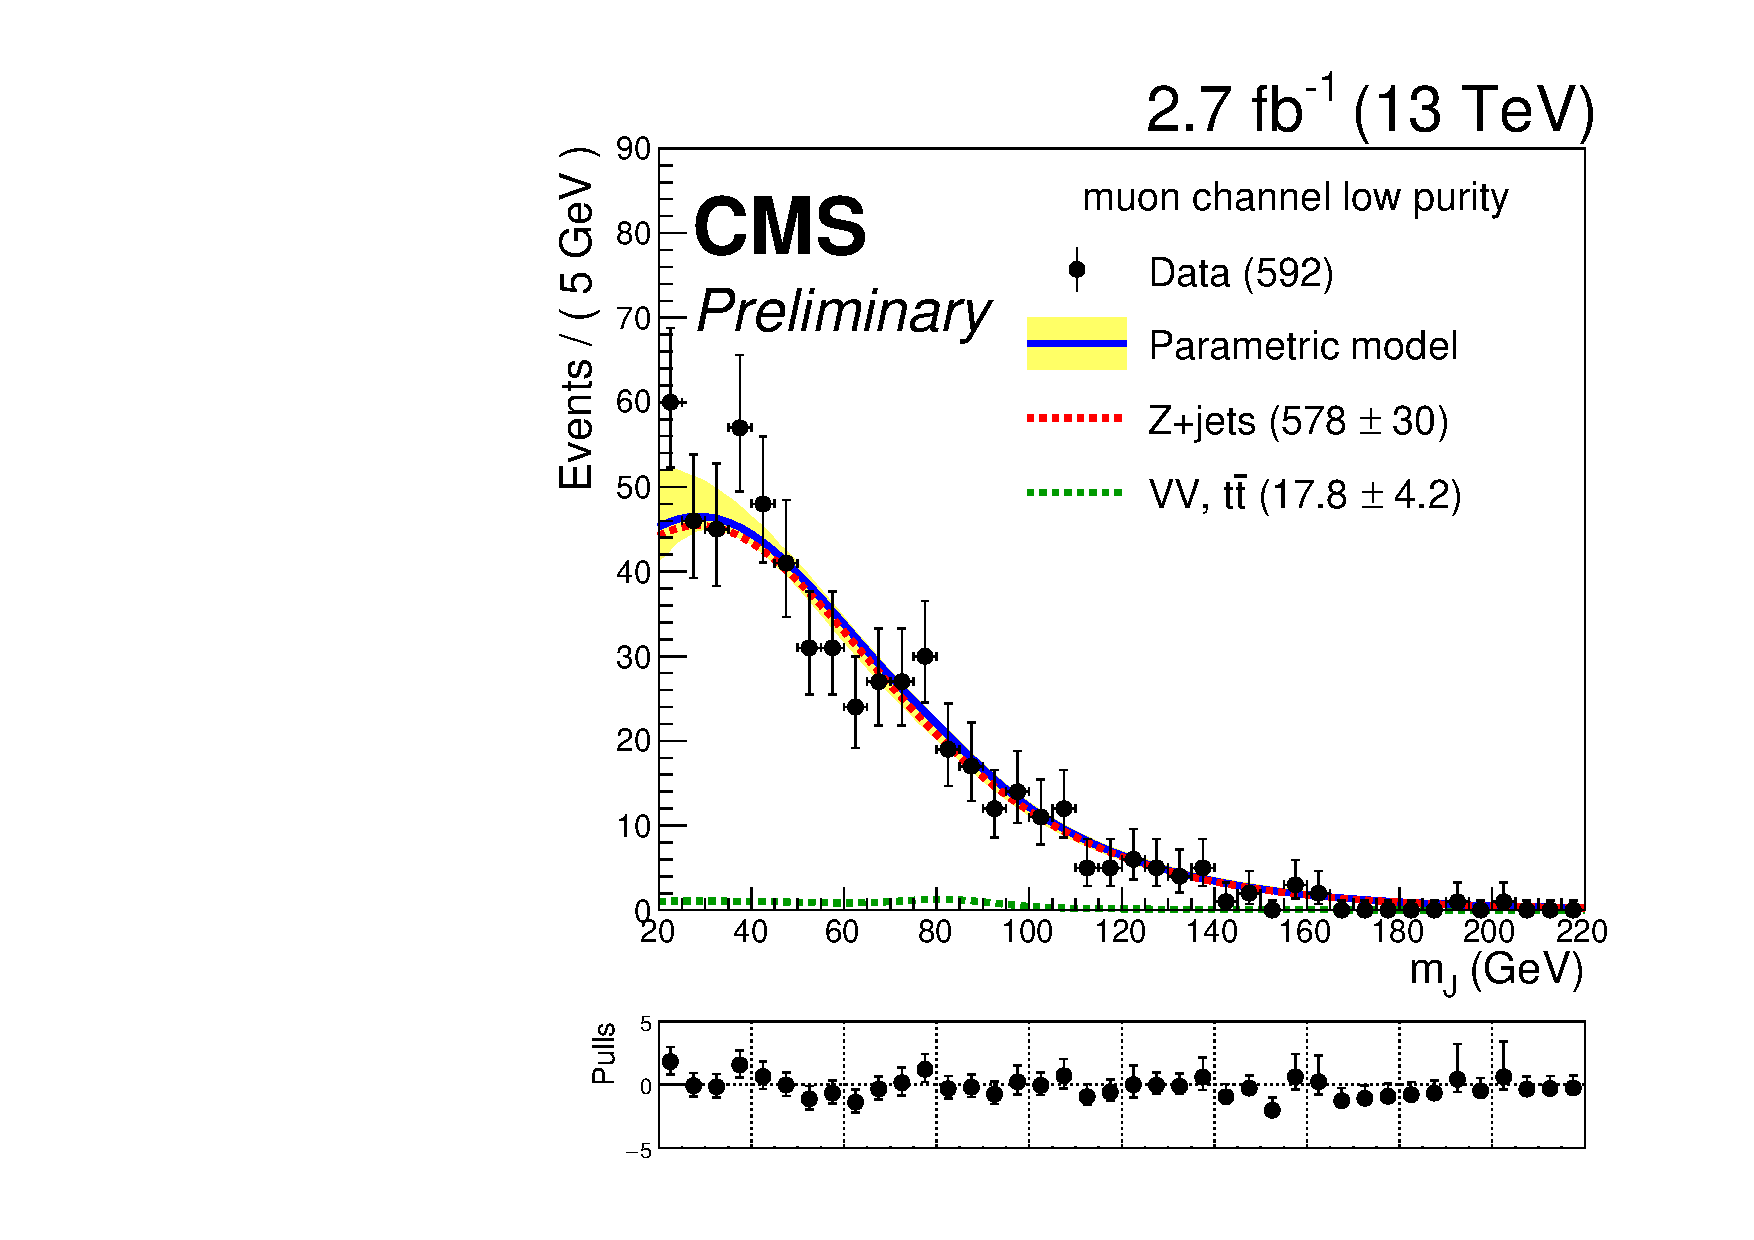
\includegraphics[width=0.39\linewidth]{mjFitMLP.pdf}
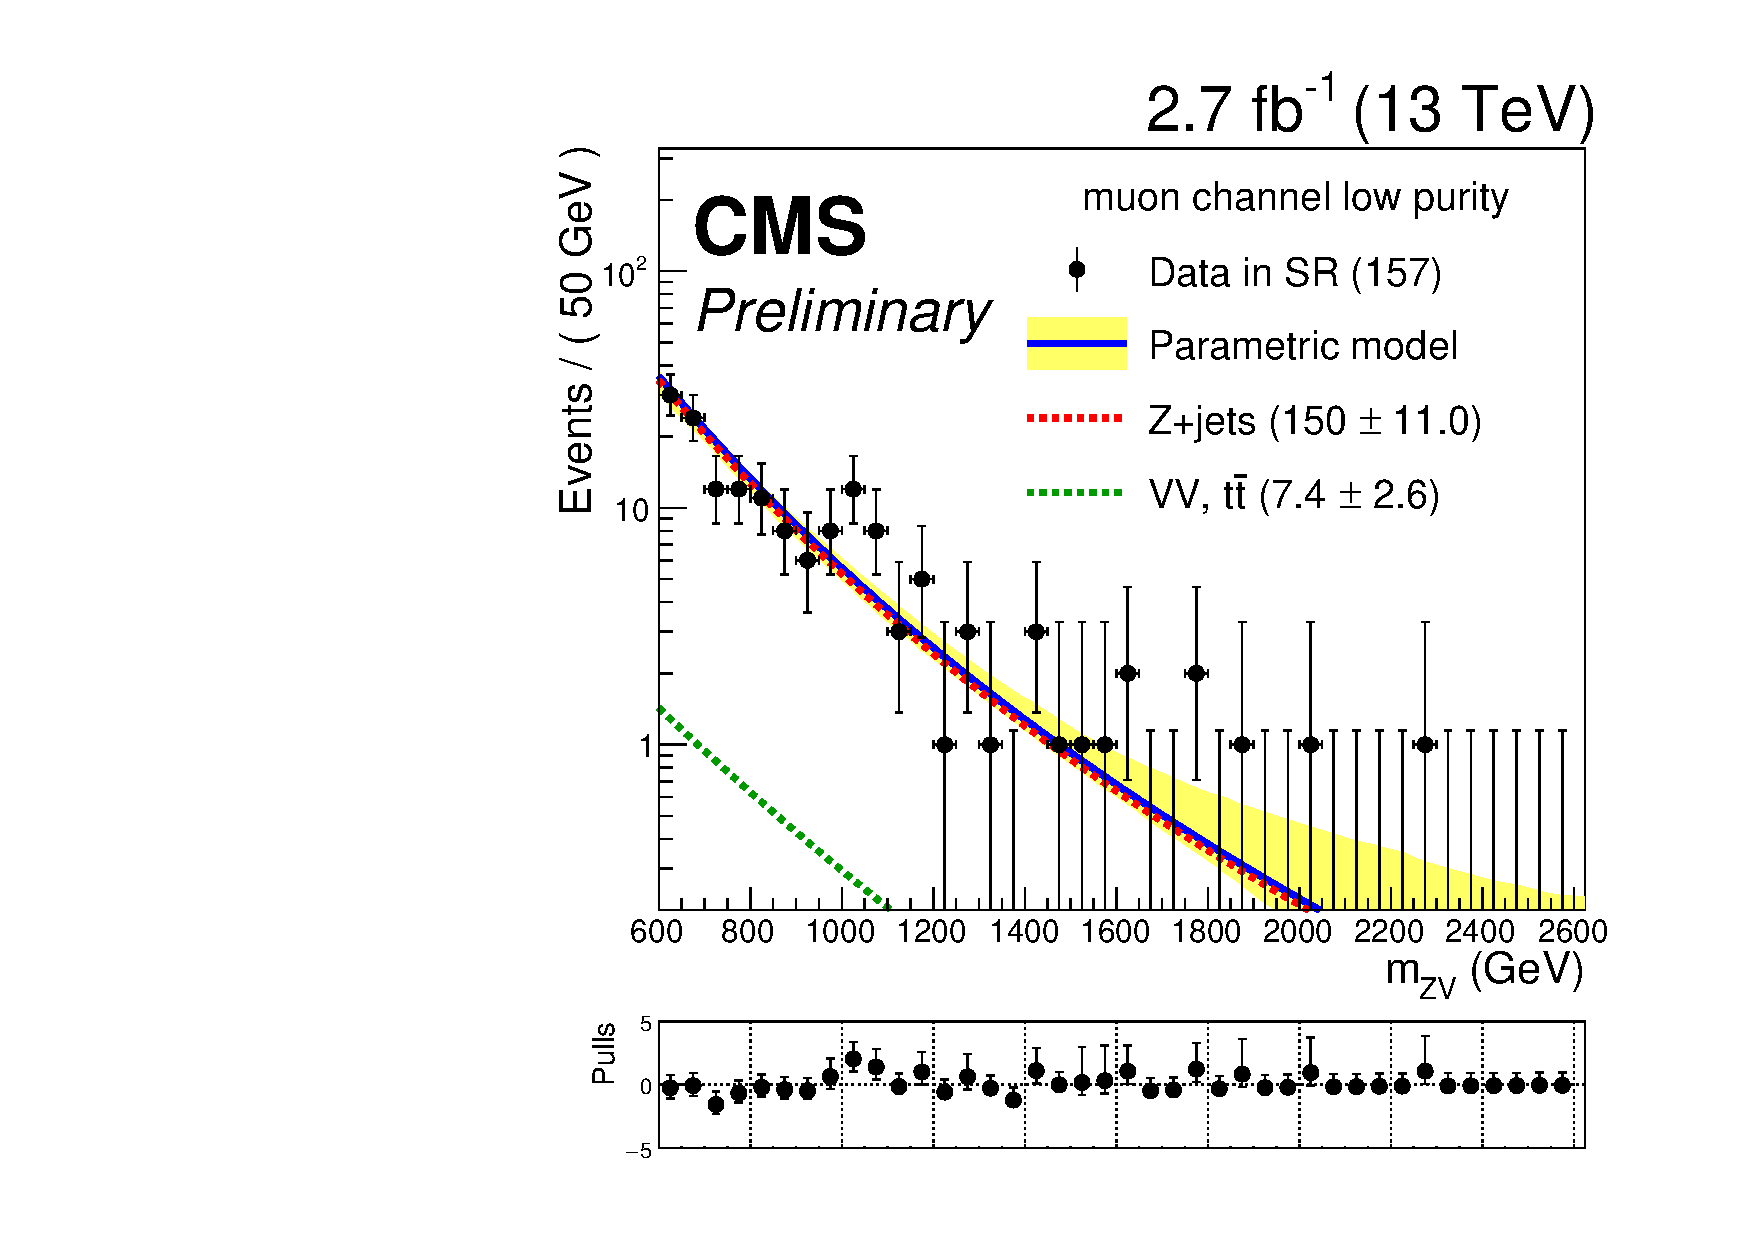
\includegraphics[width=0.39\linewidth]{mVZsigMLP.pdf}\\
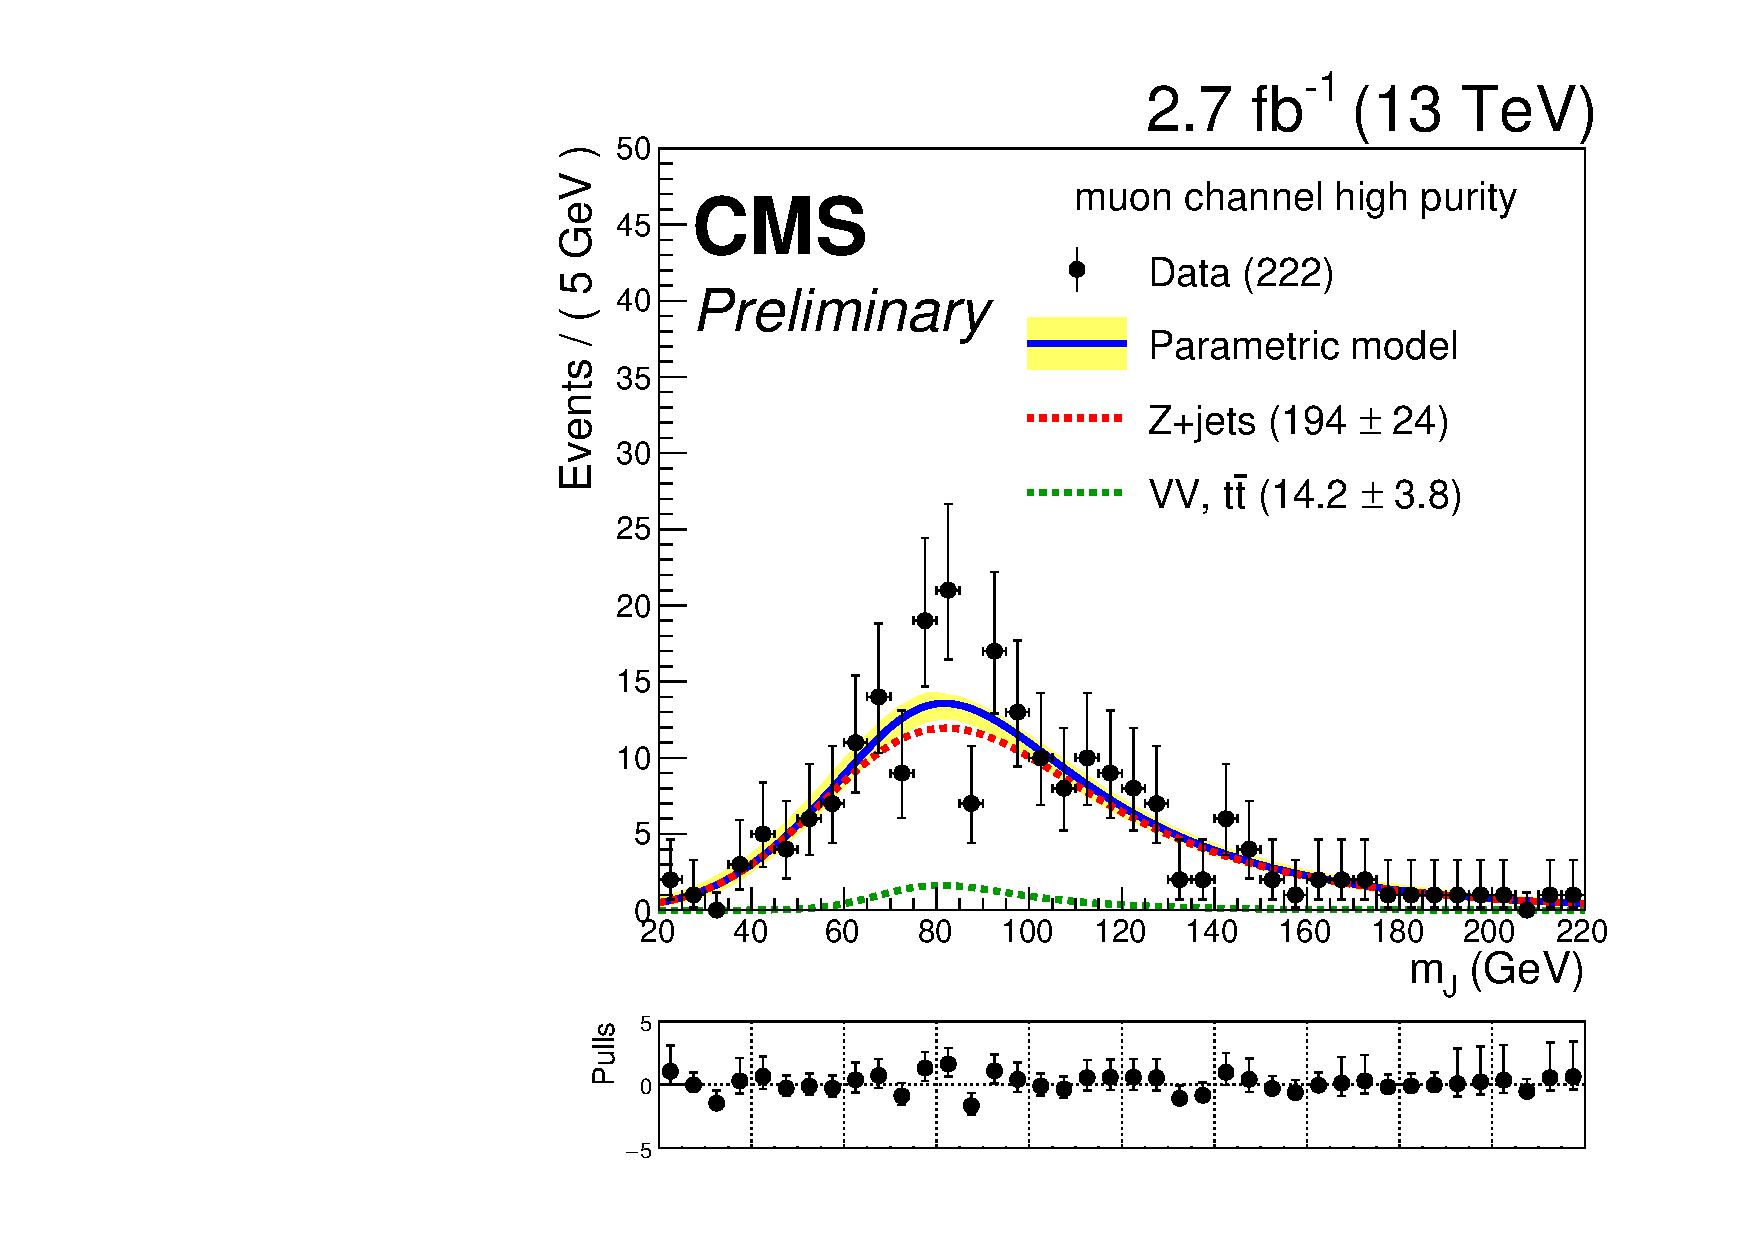
\includegraphics[width=0.39\linewidth]{mjFitMHP.pdf}
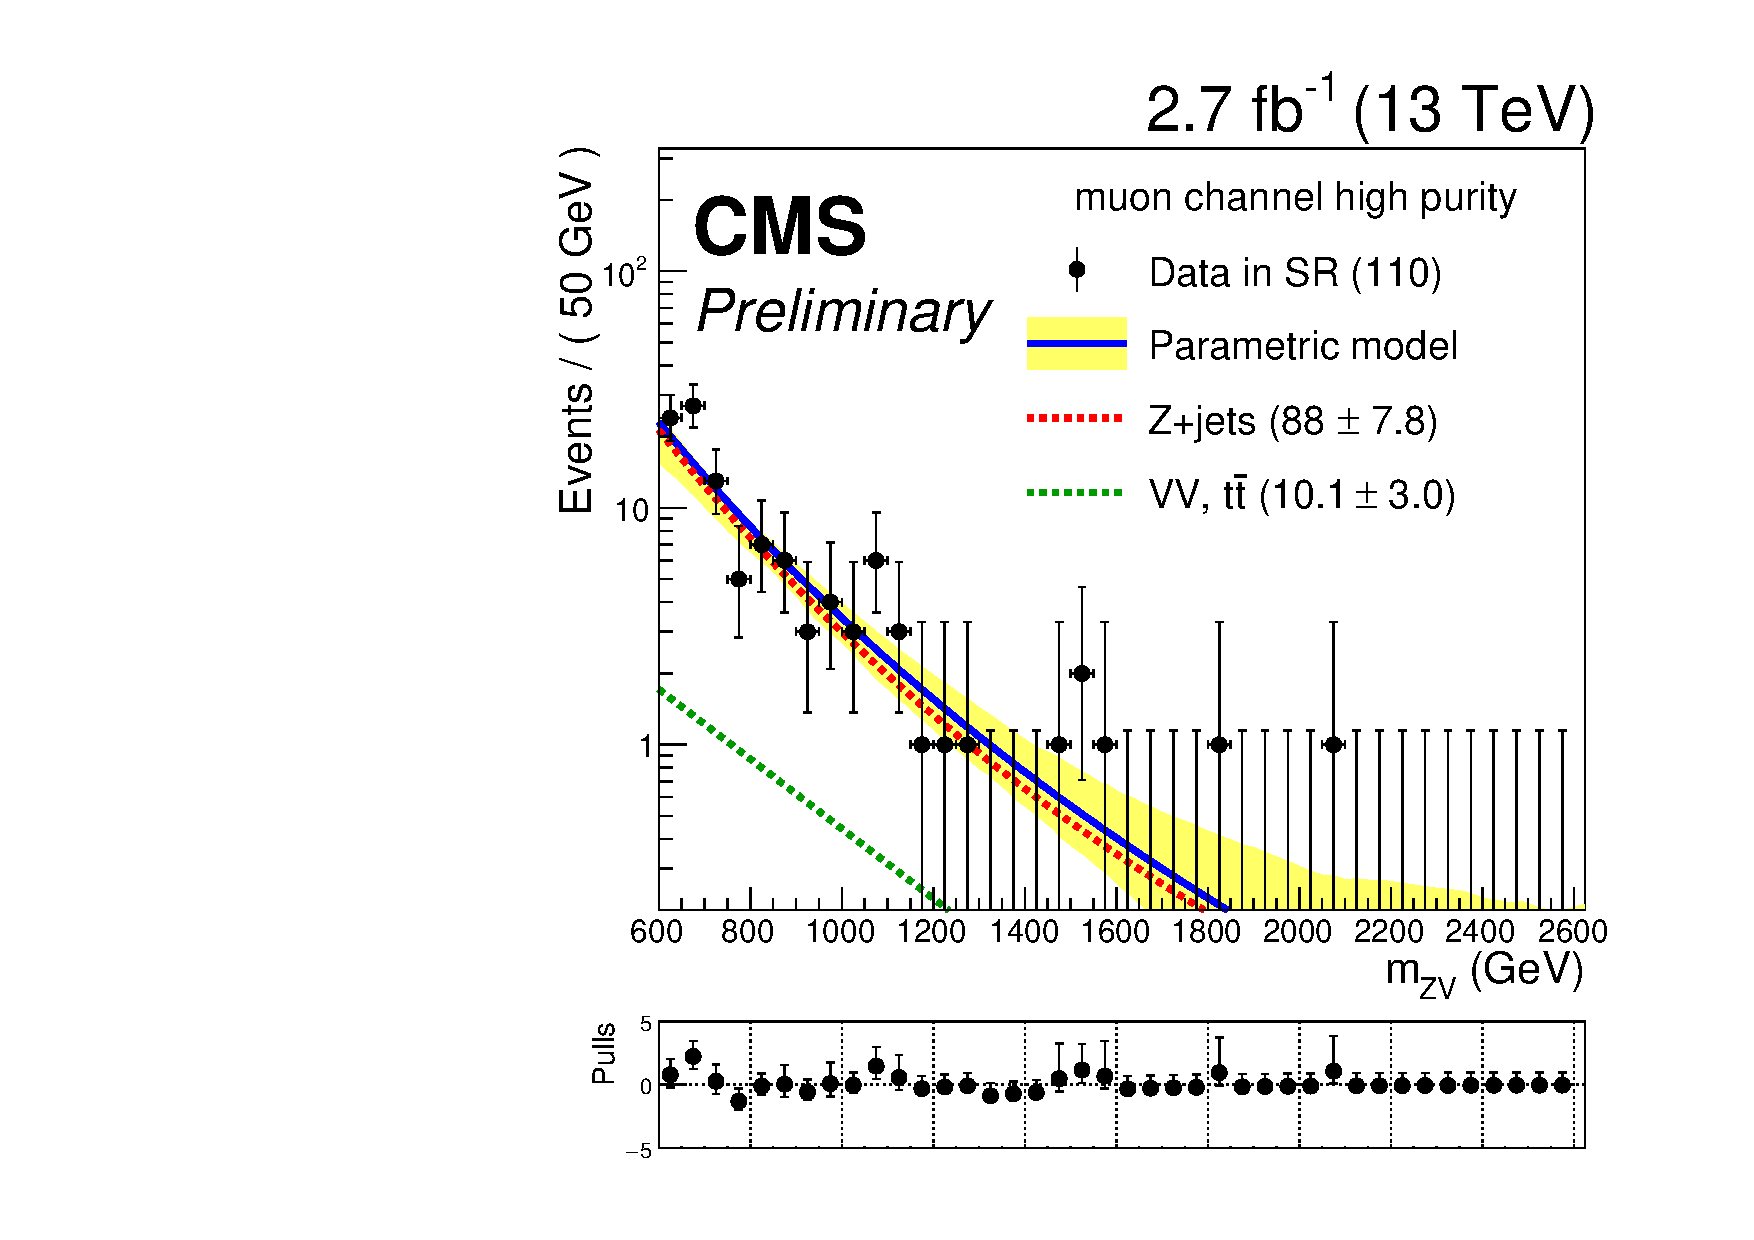
\includegraphics[width=0.39\linewidth]{mVZsigMHP.pdf}
\caption{
Jet mass (left) and invariant mass $m_{\rm ZV}$ (right) distributions for the low purity (top) and high purity (bottom) categories, in the muon channel.
}
\label{fig:jetmass}
\end{center}
\end{figure}

\section{Conclusions}
Upper limits on the cross section $\sigma($G$_{\rm bulk}\rightarrow ZZ$) as function of the resonance mass are shown in Fig. \ref{fig:limit}. The results obtained are compatible with the standard model prediction in the explored mass range. Given the low statistics in data and the low cross section of the bulk graviton model, the present analysis \cite{CMS:PAS:B2G16010} did not reach the sensitivity required to establish exclusion limits on the theoretical cross section (red line in Fig. \ref{fig:limit}).

In the low mass search, an excess at 650 GeV is observed. The local p-value of the excess is $4.0\times 10^{-4}$, equivalent to a significance of 3.9 $\sigma$. Taking into account the look-elsewhere effect in the mass range $550 < m_{\rm ZV} < 1400$ GeV, the significance is reduced to 3.5 $\sigma$.

\begin{figure}[htb]
\begin{center}
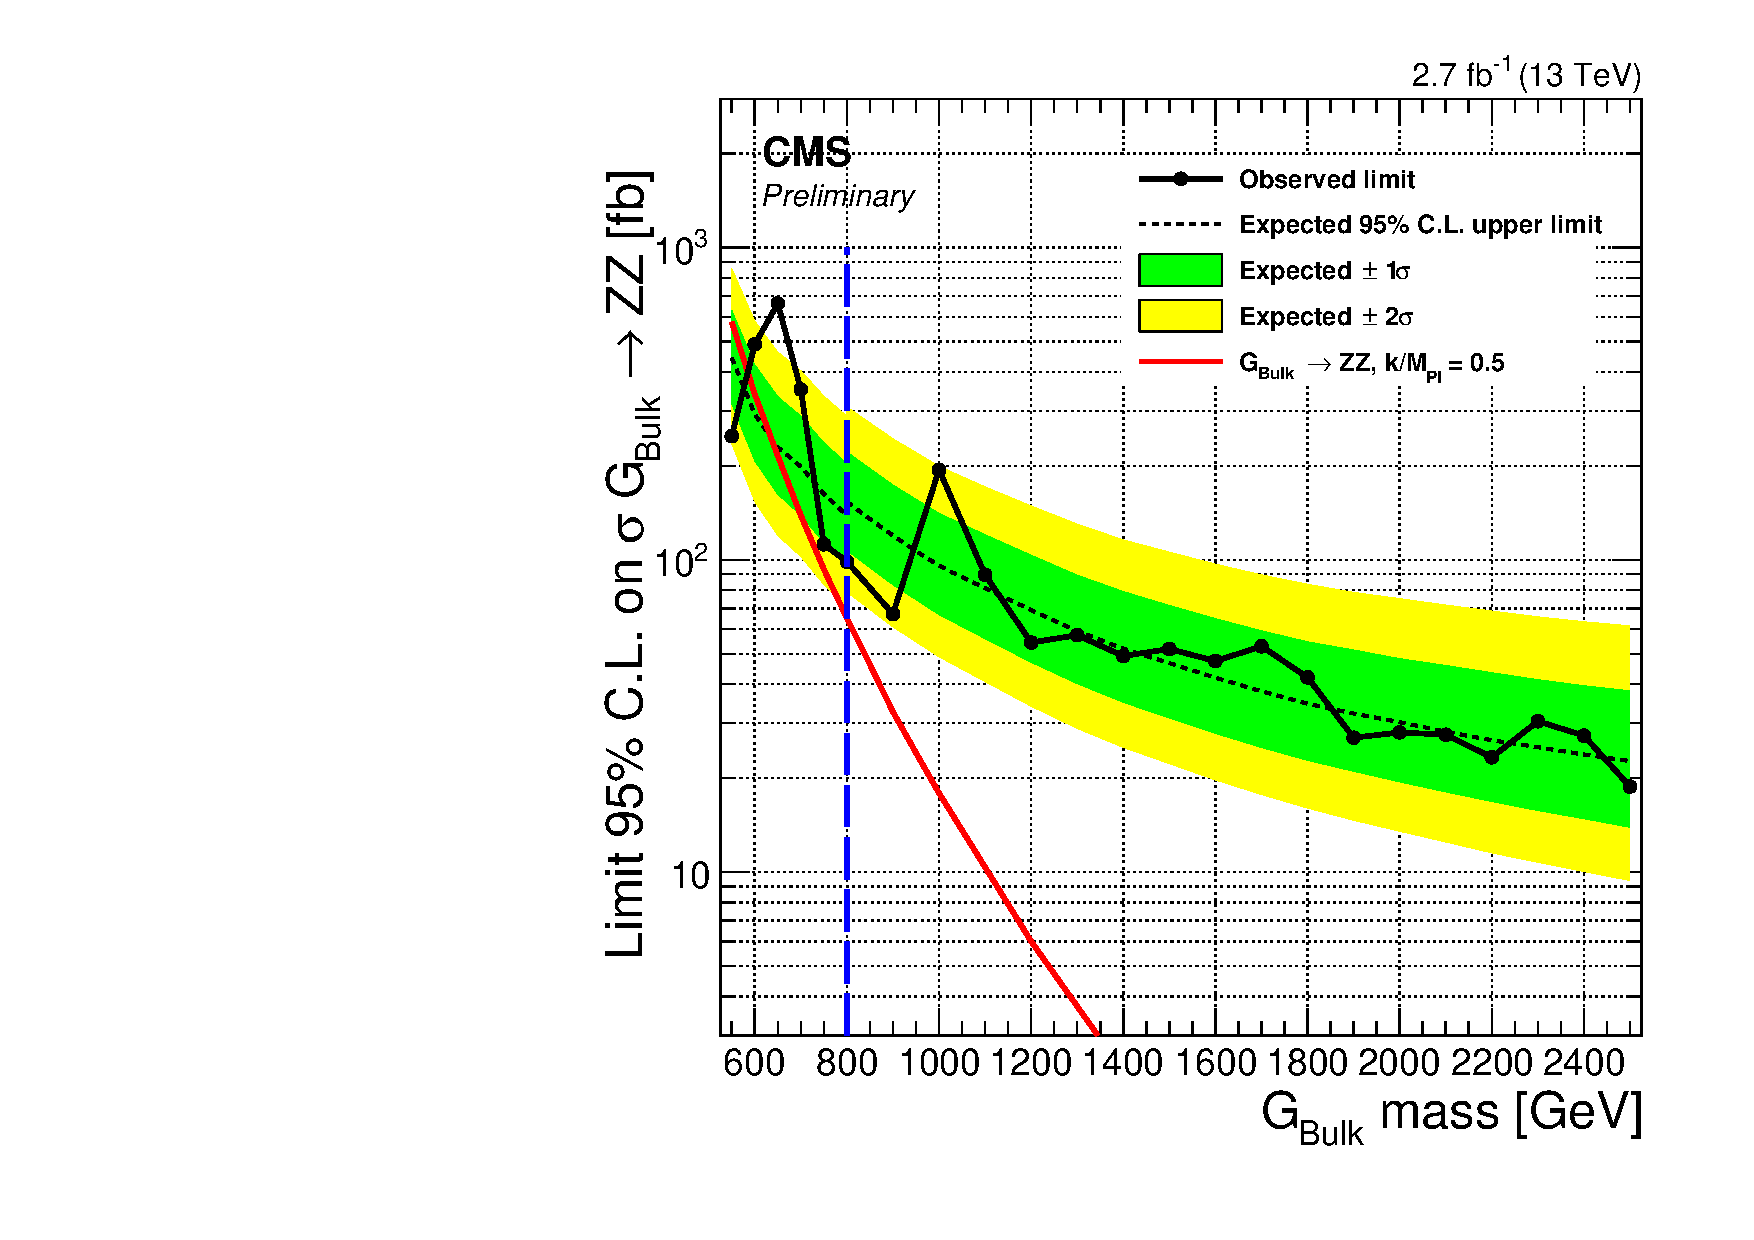
\includegraphics[width=0.45\linewidth]{combinedLimit.pdf}
\caption{
Observed and expected limits at 95\% confidence level (C.L.) on the cross section $\sigma($G$_{\rm bulk}\rightarrow ZZ$). The 68\% and 95\% ranges of expectation for the background-only model are shown with green and yellow bands, respectively. The blue line sets the boundary at 800 GeV that separates the low mass and high mass searches.
}
\label{fig:limit}
\end{center}
\end{figure}

\begin{thebibliography}{99}

\bibitem{Randall:1999ee} L. Randall and R. Sundrum, \emph{A large mass hierarchy from a small extra dimension, Phys. Rev. Lett.} {\bf 83} (1999) 3370 [hep-ph/9905221]. 

\bibitem{Randall:1999vf} L. Randall and R. Sundrum, \emph{An alternative to compactification, Phys. Rev. Lett.} {\bf 83} (1999) 4690 [hep-ph/9906064]. 

%\bibitem{Fitzpatrick:2007qr} A. L. Fitzpatrick, J. Kaplan, L. Randall, and L. T. Wang, {\it Searching for the Kaluza-Klein graviton in bulk RS models, JHEP} {\bf 09} (2007) 013 [hep-ph/0701150].

\bibitem{Chatrchyan:2008aa} CMS Collaboration, \emph{The CMS experiment at the CERN LHC, JINST} {\bf 3} (2008) S08004.

\bibitem{Ellis:2009su} S. D. Ellis, C. K. Vermilion, and J. R. Walsh, \emph{Techniques for improved heavy particle searches with jet substructure, Phys. Rev.  D} {\bf 80} (2009) 051501 [hep-ph/0903.5081]

\bibitem{Thaler:2011gf} J. Thaler and K. Van Tilburg, \emph{Maximizing Boosted Top Identification by Minimizing N-subjettiness, JHEP} {\bf 02} (2012) 093 [hep-ph/1108.2701]

\bibitem{CMS:PAS:B2G16010}CMS Collaboration, \emph{Search for diboson resonances in the semileptonic $\mathrm{X}\rightarrow\mathrm{Z}\mathrm{V}\rightarrow\ell^+\ell^-~\mathrm{q\bar{q}}$ final state at $\sqrt{s} = 13~\mathrm{TeV}$ with CMS}, CMS-PAS-B2G-16-010 (2016)




\end{thebibliography}

\end{document}
